\pdfminorversion=4
\documentclass[aspectratio=169]{beamer}

\mode<presentation>
{
  \usetheme{default}
  \usecolortheme{default}
  \usefonttheme{default}
  \setbeamertemplate{navigation symbols}{}
  \setbeamertemplate{caption}[numbered]
  \setbeamertemplate{footline}[frame number]  % or "page number"
  \setbeamercolor{frametitle}{fg=white}
  \setbeamercolor{footline}{fg=black}
} 

\usepackage[english]{babel}
\usepackage[utf8x]{inputenc}
\usepackage{tikz}
\usepackage{courier}
\usepackage{array}
\usepackage{bold-extra}
\usepackage{minted}
\usepackage[thicklines]{cancel}
\usepackage{fancyvrb}

\xdefinecolor{dianablue}{rgb}{0.18,0.24,0.31}
\xdefinecolor{darkblue}{rgb}{0.1,0.1,0.7}
\xdefinecolor{darkgreen}{rgb}{0,0.5,0}
\xdefinecolor{darkgrey}{rgb}{0.35,0.35,0.35}
\xdefinecolor{darkorange}{rgb}{0.8,0.5,0}
\xdefinecolor{darkred}{rgb}{0.7,0,0}
\definecolor{darkgreen}{rgb}{0,0.6,0}
\definecolor{mauve}{rgb}{0.58,0,0.82}

\title[2022-02-08-jlab-roundtable-language-history]{History and Adoption of Programming Languages in NHEP}
\author{Jim Pivarski}
\institute{Princeton University -- IRIS-HEP}
\date{February 8, 2202}

\usetikzlibrary{shapes.callouts}

\begin{document}

\logo{\pgfputat{\pgfxy(0.11, 7.4)}{\pgfbox[right,base]{\tikz{\filldraw[fill=dianablue, draw=none] (0 cm, 0 cm) rectangle (50 cm, 1 cm);}\mbox{\hspace{-8 cm}
\includegraphics[height=1 cm]{princeton-logo-long.png}\hspace{0.1 cm}\raisebox{0.1 cm}{
\includegraphics[height=0.8 cm]{iris-hep-logo-long.png}}\hspace{0.1 cm}}}}}

\begin{frame}
  \titlepage
\end{frame}

\logo{\pgfputat{\pgfxy(0.11, 7.4)}{\pgfbox[right,base]{\tikz{\filldraw[fill=dianablue, draw=none] (0 cm, 0 cm) rectangle (50 cm, 1 cm);}\mbox{\hspace{-8 cm}
\includegraphics[height=1 cm]{princeton-logo.png}\hspace{0.1 cm}\raisebox{0.1 cm}{
\includegraphics[height=0.8 cm]{iris-hep-logo.png}}\hspace{0.1 cm}}}}}

% Uncomment these lines for an automatically generated outline.
%\begin{frame}{Outline}
%  \tableofcontents
%\end{frame}

% START START START START START START START START START START START START START

% We are planning the meetings for 2022 and we would like to organise a meeting focused on the programming languages that are used in the community. The idea is to cover a history of languages and their adoption, the modern C++ ecosystem and take a look at Julia as well. We wanted to invite you to give a 20’ talk on the history and adoption of languages in NHEP, building on talks you gave before and (IMO) covering things like the early use and deprecation of Fortran, the rise of C++ and the adoption of Python as an equally important language in the community (of course, you have the freedom to focus on what you would like).

\begin{frame}{\mbox{ }}
\large
\vspace{0.5 cm}
This talk is a historical overview of programming languages widely used in NHEP, especially what motivated each language's adoption.

\vspace{1 cm}
\uncover<2->{There have always been physicists at the edge, trying out new languages, but most physicists have only ever used one or two; the field is slow to change.}

\vspace{1 cm}
\uncover<3->{\textcolor{darkblue}{Thesis:} (1) change motivated more by ``pain points'' than incremental benefits,}

\vspace{0.2 cm}
\uncover<4->{\phantom{Thesis:}\hspace{0.035 cm} (2) hysteresis matters: first ``good enough'' solution wins.}
\end{frame}

\begin{frame}{Three major transitions (so far)}
\begin{columns}
\column{1.1\linewidth}
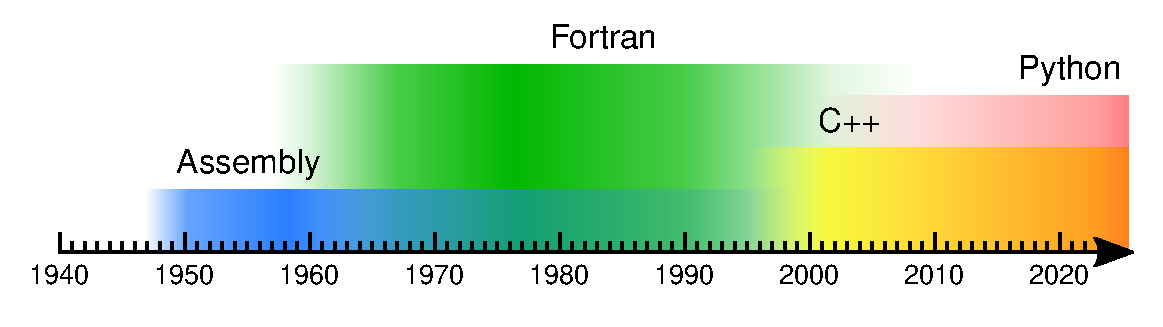
\includegraphics[width=\linewidth]{PLOTS/programming-languages.pdf}
\end{columns}

\large
\vspace{0.5 cm}
Adoption of

\begin{description}
\item[\textcolor{black}{Fortran:}] \textcolor{darkblue}{immediate;} \textcolor{darkgreen}{for syntax and portability;} \textcolor{violet}{no infrastructure to replace}
\item[\textcolor{black}{C++:}] \textcolor{darkblue}{long overdue;} \textcolor{darkgreen}{for data structures;} \textcolor{violet}{replaced infrastructure in a burst}
\item[\textcolor{black}{Python:}] \textcolor{darkblue}{slowly overtook the alternatives;} \textcolor{darkgreen}{for interactivity;} \textcolor{violet}{different niche}
\end{description}
\end{frame}

\begin{frame}{NHEP was an early adopter of digital computers}
\Large
\vspace{0.35 cm}
\begin{columns}
\column{1.05\linewidth}
One of the very first applications was Monte Carlo (neutron transport).

\vspace{-0.2 cm}
\begin{center}
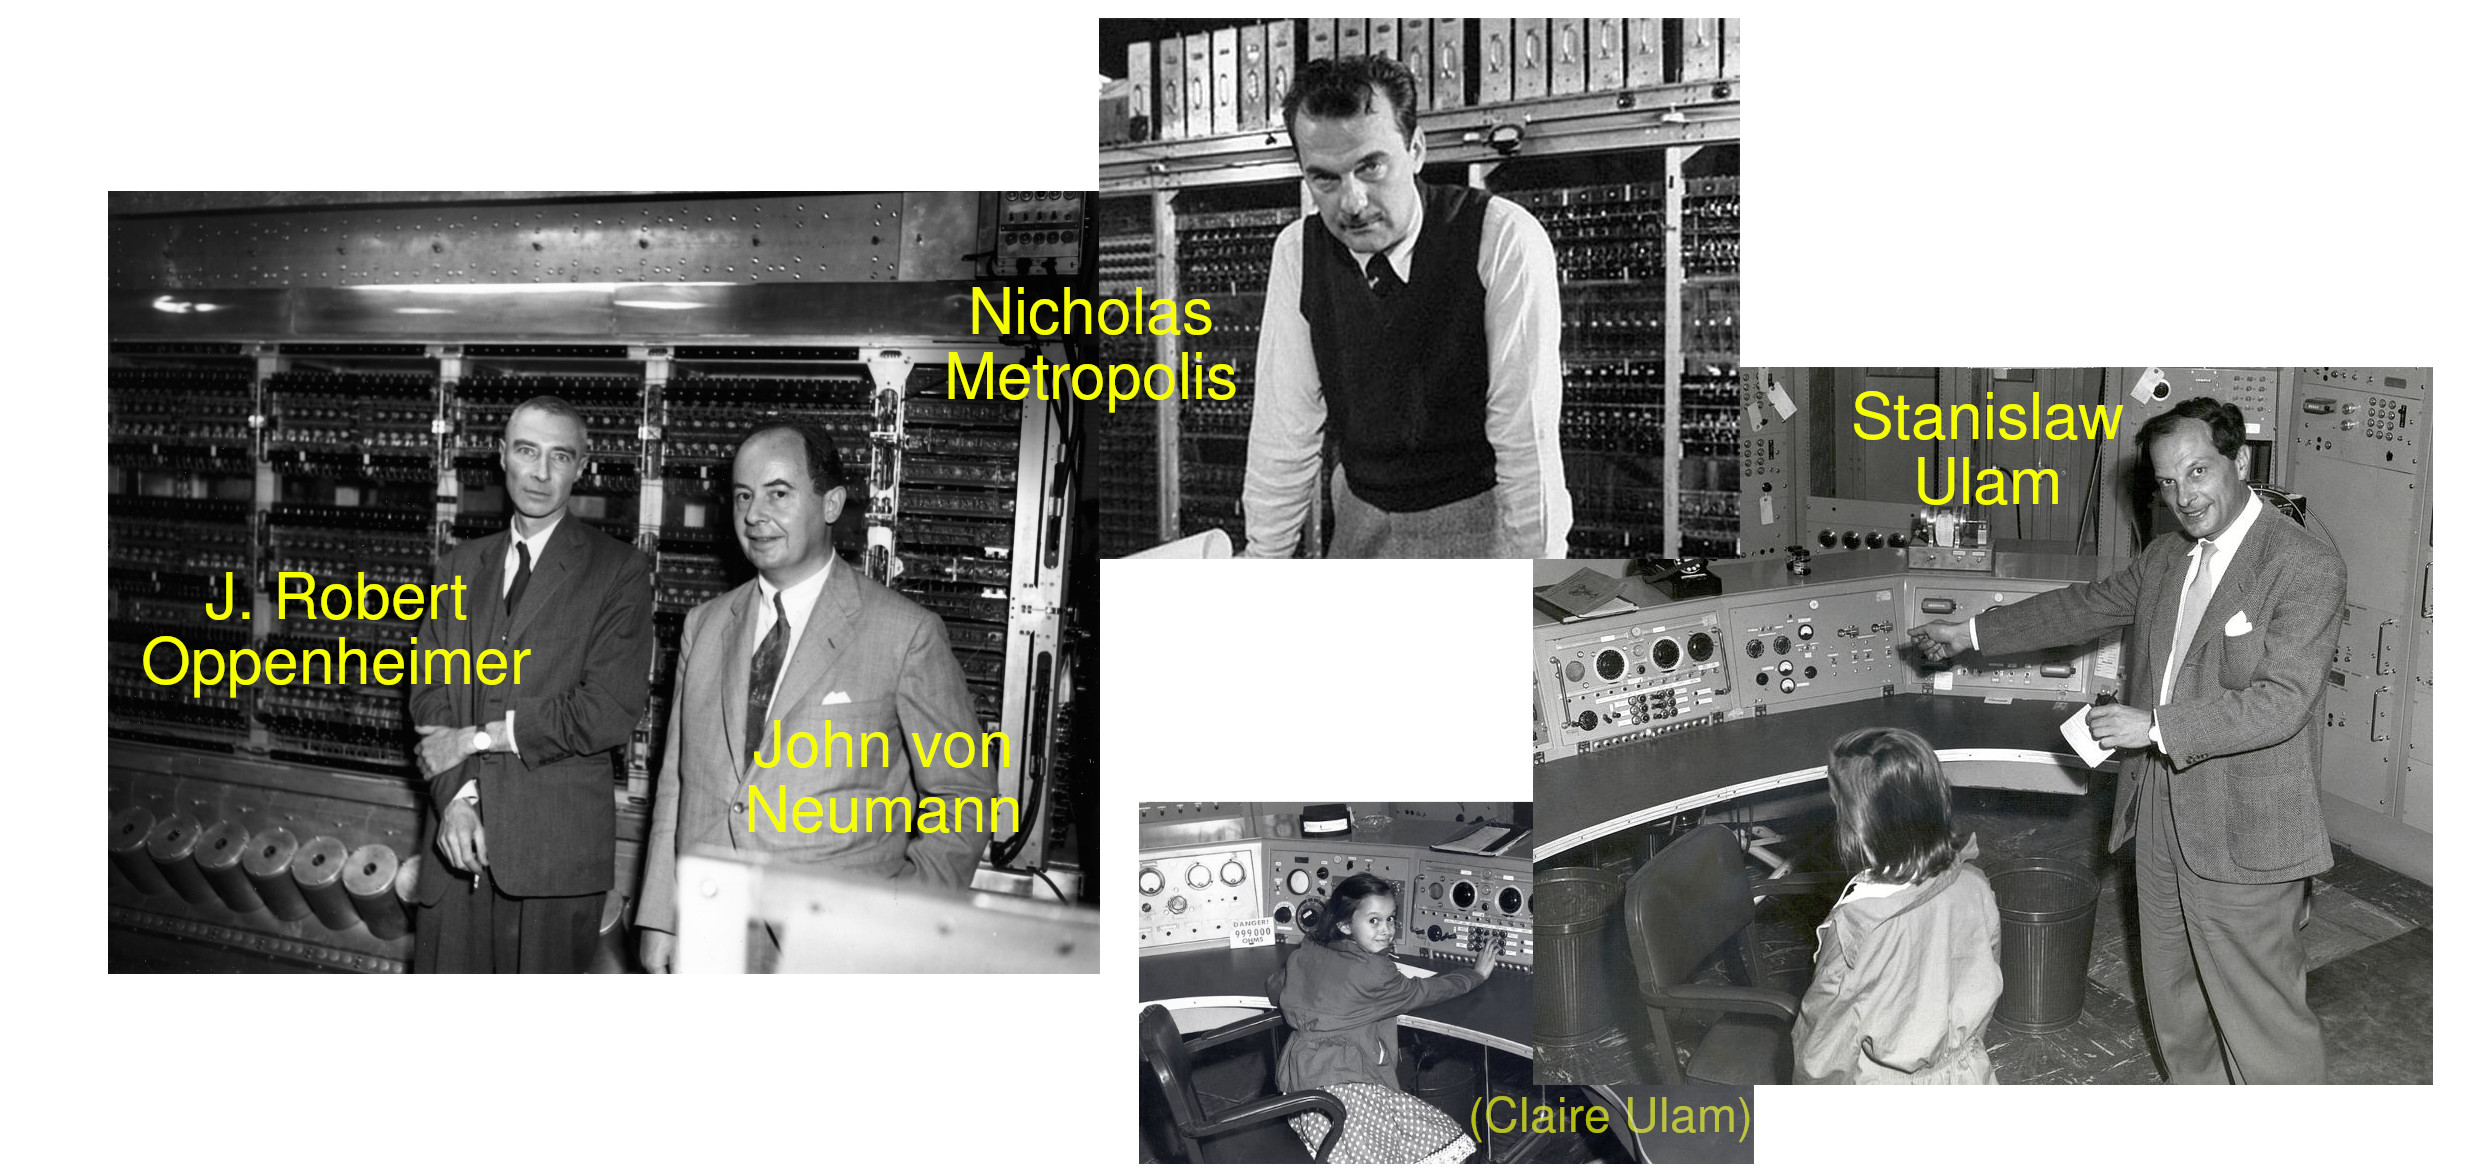
\includegraphics[width=0.78\linewidth]{PLOTS/manhattan-project-physicists-and-computer.jpg}
\end{center}
\end{columns}
\end{frame}

\begin{frame}{And so was data analysis}
\vspace{0.5 cm}
\textcolor{darkblue}{Example:} Luis Alvarez's group at the Bevatron: \textcolor{darkgreen}{\$2M} bubble chamber, \textcolor{darkgreen}{\$0.2M} IBM 650

\vspace{0.25 cm}
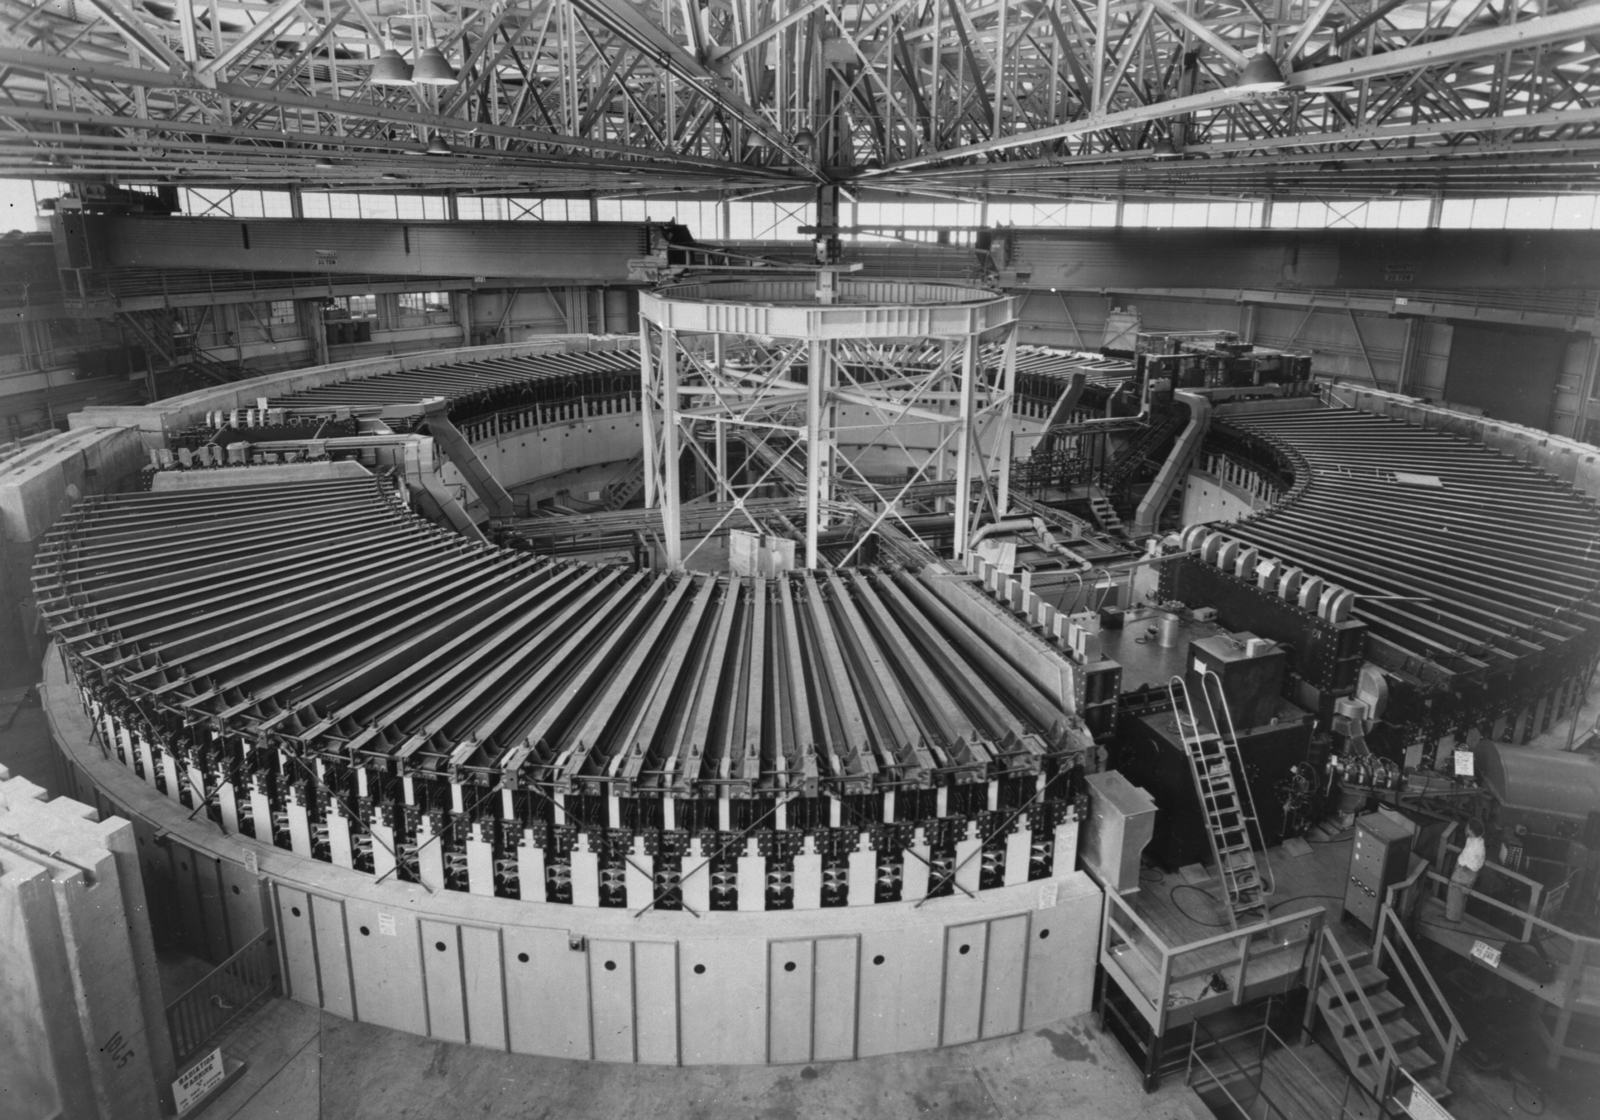
\includegraphics[width=0.45\linewidth]{PLOTS/overall-view-of-bevatron-magnet-photograph-taken-september-6-1955-bevatron-088cb0-1600.jpg}\hfill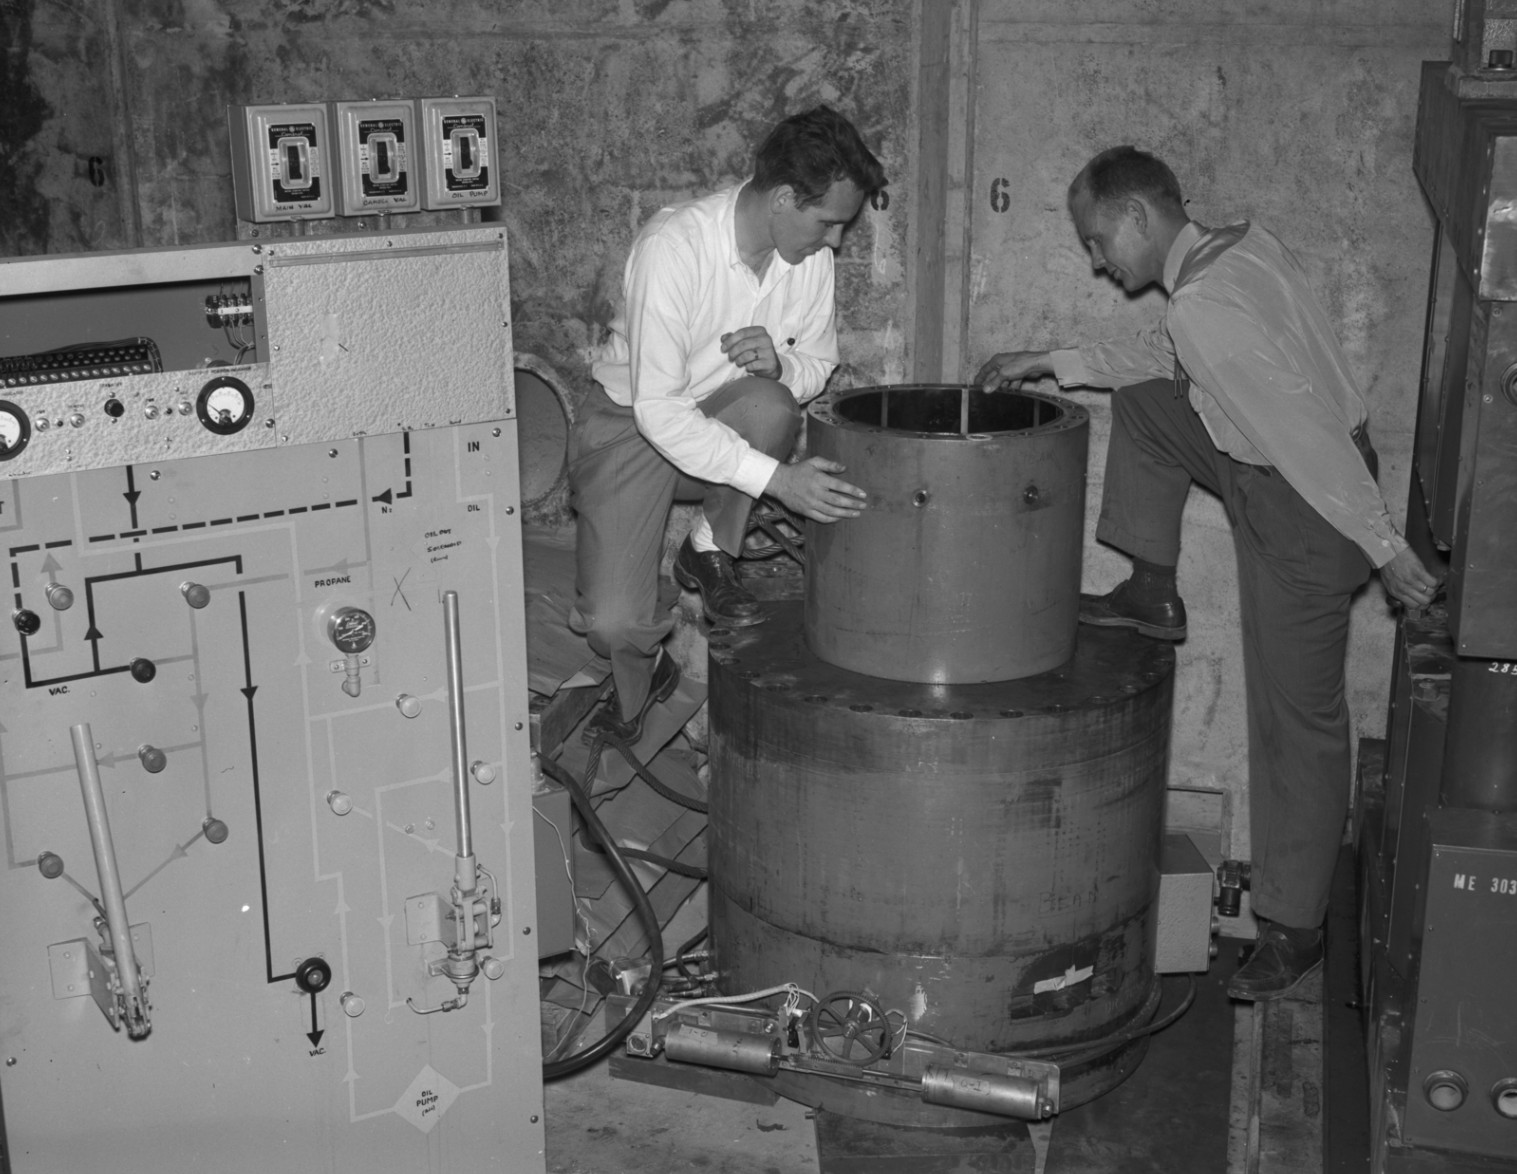
\includegraphics[width=0.5\linewidth]{PLOTS/alvarez-group-bubble-chamber.jpg}
\end{frame}


\end{document}
